\documentclass[11pt,a4paper,twocolumn]{article}

\usepackage[margin=.75in]{geometry}
\usepackage{indentfirst}
\usepackage{listings}
\usepackage{color}
\usepackage{hyperref}
\usepackage[super]{nth}
\usepackage{siunitx}
\usepackage{graphicx}
\graphicspath{ {./resources/} }
\usepackage{pgfplots}
\usepackage{pgfplotstable}
\pgfplotsset{compat=1.18}

\definecolor{dkgreen}{rgb}{0,0.6,0}
\definecolor{gray}{rgb}{0.5,0.5,0.5}
\definecolor{mauve}{rgb}{0.58,0,0.82}
\definecolor{orange}{rgb}{.7,.3,0}

\makeatletter
\lst@InstallKeywords k{types}{typestyle}\slshape{typestyle}{}ld
\makeatother

\lstnewenvironment{code-c}
{
    \lstset{
        language=c,
        aboveskip=3mm,
        belowskip=3mm,
        showstringspaces=false,
        basicstyle={\small\ttfamily},
        keywordstyle=\color{blue},
        commentstyle=\color{dkgreen},
        stringstyle=\color{mauve},
        typestyle=\color{orange},
        breaklines=true,
        breakatwhitespace=true,
        moretypes={
            LLConnection, LLConnectionParams, LLRole, Frame, ByteVector,
            uint8_t, size_t, ssize_t, bool, termios, timer_t
        }
    }
}
{}

\lstnewenvironment{code-bash}
{
    \lstset{
        language=bash,
        aboveskip=3mm,
        belowskip=3mm,
        showstringspaces=false,
        basicstyle={\small\ttfamily},
        keywordstyle=\color{blue},
        commentstyle=\color{dkgreen},
        stringstyle=\color{mauve},
        typestyle=\color{orange},
        breaklines=true,
        breakatwhitespace=true
    }
}
{}

\title{Computer Networks -- \nth{2} Project Report}
\author{João Pereira, Nuno Pereira}

\begin{document}

\maketitle

\section{Introduction}

The goal of this project was to set up a small computer network and showcase that it is correctly configured using a "download application", also developed for the purpose of this project.

\section{Download Application}

Part 1 consists in the development of a small application that downloads files using the FTP protocol as described in \href{https://www.rfc-editor.org/rfc/rfc959}{RFC959}.
It takes an argument that adopts the \textit{URL} syntax as described in \href{https://www.rfc-editor.org/rfc/rfc1738}{RFC1738}. Example:

\begin{code-bash}
download ftp://ftp.up.pt/pub/hello.txt
\end{code-bash}

where the \textit{URL} path is:

\begin{code-bash}
ftp://[<username>[:<password>]@]<host>[:<port>]/<path>
\end{code-bash}

This allowed us to learn things such as:
\begin{itemize}
    \item UNIX utilities for handling \textit{URL}s like \textit{getaddrinfo()};
    \item Searching, reading and interpreting RFCs, like the one that describes de FTP protocol;
    \item UNIX utilities to communicate with remote services like sockets;
    \item how to develop a simple FTP client in C;
    \item DNS peculiarities when developing a network-driven application;
\end{itemize}

\subsection{Architecture of the download application}

The download application's flow consists of a series of steps, as follows:
\begin{enumerate}
    \item Parsing the \textit{URL} string given as the argument to the program to extract the various fragments that make up the \textit{URL} such as the host name or the path of the file to download.
    \item Connecting to the supplied host on the specified port (defaults to 21, the standard FTP control port).
    \item Entering passive mode and receiving the data connection's host and port information.
    \item Connecting to the data connection's host and port.
    \item Signaling that the remote server should start the transfer of the file specified in the \textit{path} portion of the \textit{URL} string.
    \item Reading a data buffer from the data connection and writing that to a local file whose name is the same as the one being transferred.
    \item Closing the connection.
\end{enumerate}

Network communication is mediated by TCP sockets.
Making use of the custom \textit{URL} parser and \textit{getaddrinfo()}, the FTP server's IP and control port are obtained (the control port defaults to 21 as per the FTP protocol standard).

A TCP connection is established and the program starts sending commands through the control connection. All lines that are/will be sent back by the server are parsed and the given response code is extracted: if the code does not match what is expected, the program terminates with a status code of -1.

The program performs a login against the remote server (if no username is given in the \textit{URL} string then an anonymous login is attempted).

Next, passive mode is entered: in case of success the server responds with \textbf{227 Entering Passive Mode (h1,h2,h3,h4,p1,p2)}, where \textbf{h1} through \textbf{h4} are the host's IP address bytes from highest to lowest and \textbf{p1} and \textbf{p2} are, respectively, the high byte and low byte of the port to connect to.

After a data connection is established, the \textit{retr} command is sent and afterwards the program starts reading buffers of data from the data connection to a file with the same name as the one being downloaded.

After all these steps, the connection is closed and the program terminates.

\subsection{Successful download}

The log of a successful download is attached as annex;

\section{Network Configuration and Analysis}

The main purpose of this part of the project was to setup a small computer network to allow a computer that normally does not have internet access to download a file from a remote server using the FTP client developed in the first part of the project.

This was accomplished by performing a series of small steps leading up the creation of the complete network, which consists of 2 "leaf" computers, 2 VLANs implemented on a Switch, a \nth{3} computer serving as a router between both VLANs and finally a commercial network router to provide internet access through the lab's own network.

All experiments were made on bench 6 of Lab 2.

\subsection{Experiment 1}

\subsubsection{Network Architecture}

At the end of the experiment, the network configuration should consist of tux63 and tux64 connected by a bridge (bridge0) through the MicroTik switch, as follows:

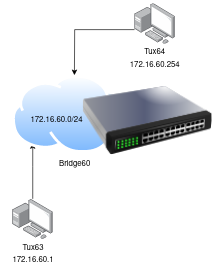
\includegraphics{experiment1}

\subsubsection{Experiment Objectives}
\subsubsection{Main Configuration Commands}
\subsubsection{Log analysis}

\subsection{Experiment 2}

\subsection{Experiment 3}

\subsection{Experiment 4}

\subsection{Experiment 5}

\subsection{Experiment 6}

\section{Conclusions}

\onecolumn
\appendix
\section{Appendix}

\subsection{Code}

\noindent In folder \lstinline{src/}.

\end{document}
